
If an matrix style display is used with a microcontroller, there are a lot of different ways to draw graphical elements. This section covers only the ways used in this project. 

\subsubsection{Matrix displays}

Since most displays produced have an rectangular shape the amount of pixel they hold is calculated like the surface of an rectangular. The number of pixels on both axis are multiplied and we get the total amount of pixels we have to manipulate. So it is obvious that the memory size of an picture explodes with its resolution. As an example we take a display with a pixel ratio of $1200 \times 825$ and a colour depth of 24 bit. We get $1200\cdot825=990'000$ pixel and $1200\cdot825\cdot24=23'760'000$ bits we have to handle. This is a huge amount of data to process with a microcontroller. \textbf{etwas über industrie schreiben wiso wir diplay treiber bausteine haben und nicht alles paralell machen}\\

If an display is rectangular the information of the pixels can be ordered in a matrix. The matrix is normally one or two dimensions to access the data. This matrix can be implemented as an array with one or two dimensions. The definition used for the array management and memory handling is given by the ISO C-Language standard. It specifies with the following sentences how the arrays are defined in the C-Language. 


\begin{displayquote}
	"An array type describes a contiguously allocated nonempty set of objects with a particular member object type, called the element type. The element type shall be complete whenever the array type is specified. Array types are characterized by their element type and by the number of elements in the array."
\end{displayquote}\cite{ISO/IEC9899}

The term allocated is referred as following 

\begin{displayquote}
	"The order and contiguity of storage allocated by successive calls to the aligned\_alloc, calloc, malloc, and realloc functions is unspecified. The pointer returned if the allocation succeeds is suitably aligned so that it may be assigned to a pointer to any type of object with a fundamental alignment requirement and then used to access such an object or an array of such objects in the space allocated (until the space is explicitly deallocated)."
\end{displayquote}\cite{ISO/IEC9899}

Alignment is defined with the sentence:
\begin{displayquote}
	"\textbf{Alignment} requirement that objects of a particular type be located on storage boundaries with addresses that are particular multiples of a byte address."
\end{displayquote}\cite{ISO/IEC9899}

 and shows the strict handling of the memory mapping in the C-Language. Since the alignment needs to be given for arrays the amount of dimensions of the array have no influence how the information is stored in the memory. In the Figure \ref{theory:matrix} the one dimensional matrix style is shown. To access this kind of display the address of the $176$-pixels reaches from $0$ to $175$ this is display can be addressed with 
 
 $$n = \lfloor \log_{2}(176) \rfloor = 8$$
 bit.   

\begin{figure}[H]
	\centering
	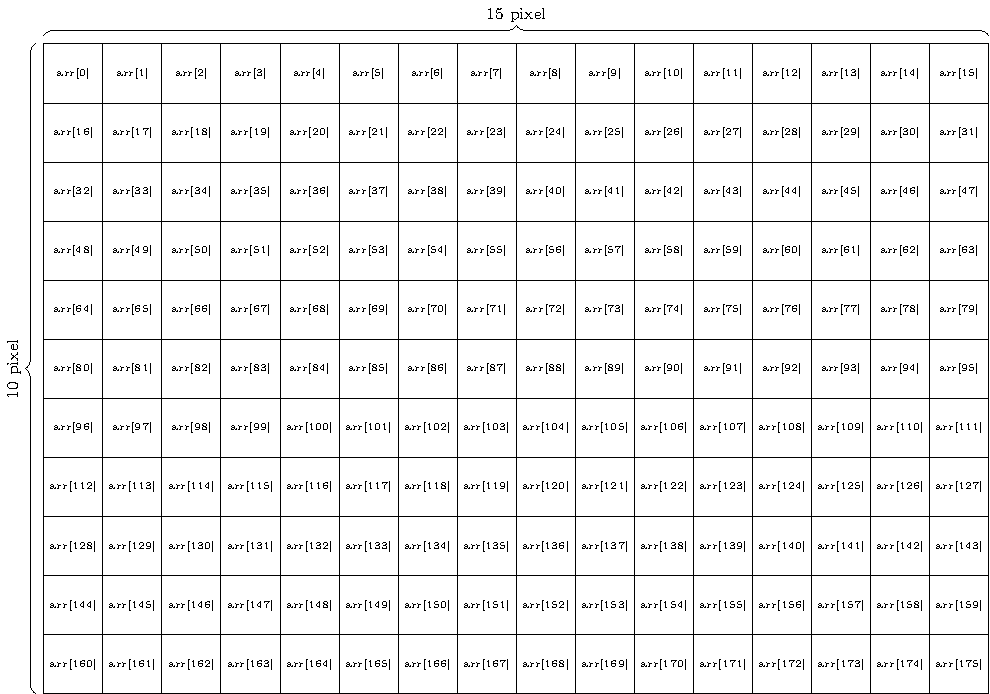
\includegraphics[width=1\textwidth]{2-theory/drawing-graphics/graphics/matrix.pdf}
	\caption{$16\times 11$ pixel display with a flat matrix \label{theory:matrix}}
\end{figure}

The 

\begin{figure}[H]
	\centering
	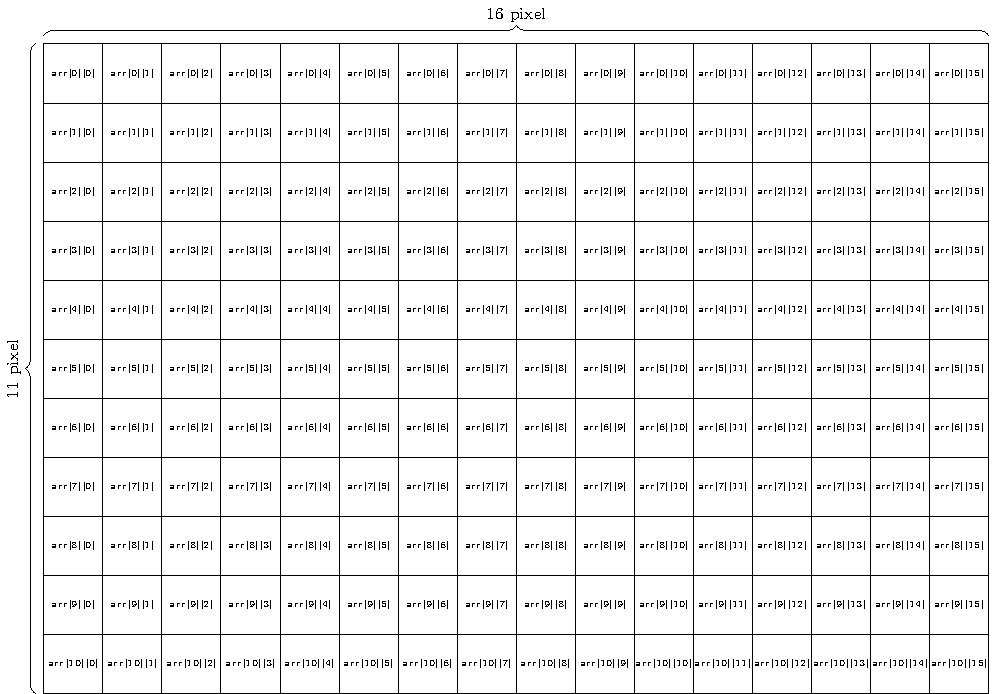
\includegraphics[width=1\textwidth]{2-theory/drawing-graphics/graphics/matrix2.pdf}
	\caption{$16\times 11$ display with a two dimensional matrix\label{theory:matrix2}}
\end{figure}

\subsubsection{Double buffering}


  

\begin{figure}[H]
	\centering
	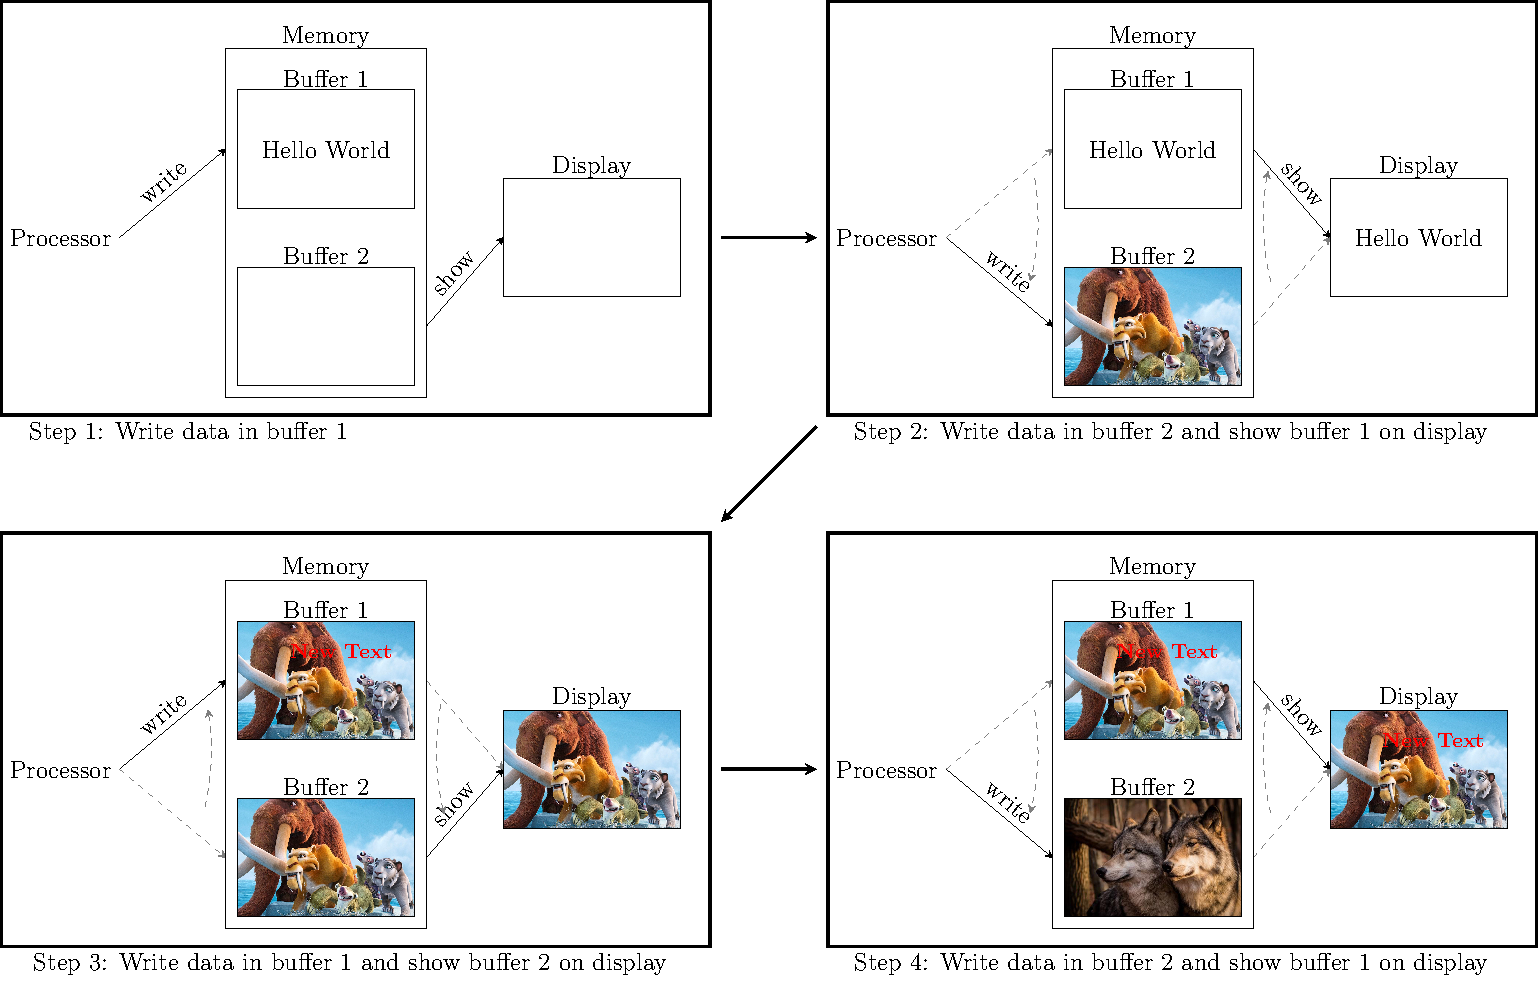
\includegraphics[width=1\textwidth]{2-theory/drawing-graphics/graphics/buffer.pdf}
	\caption{Double buffer example while writing different images to screen\label{theory:buffer}}
\end{figure}




\subsubsection{Compressed fonts}\label{chapter:CompressedFonts}

The theory shown in this chapter \ref{chapter:CompressedFonts} is only valid if the fonts used are simple fonts which are using only two different values. More complex fonts have to be compressed in a different way to avoid data loss. 
\begin{figure}[H]
	\centering
	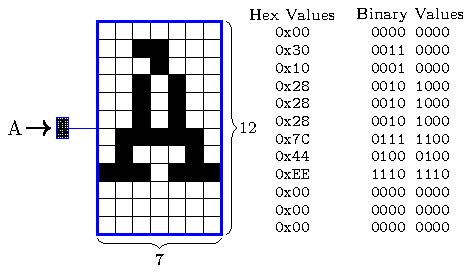
\includegraphics[width=0.8\textwidth]{2-theory/drawing-graphics/graphics/font12.pdf}
	\caption{Creation of a simple seven to twelve pixel sized font\label{theory:font12}}
\end{figure}



\subsection{Drawing text to the display}

\begin{figure}[H]
	\centering
	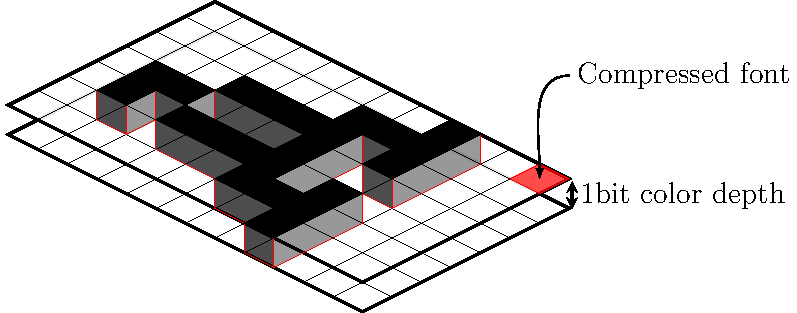
\includegraphics[width=0.6\textwidth]{2-theory/drawing-graphics/graphics/drawingfont.pdf}
	\caption{Double buffer example while writing different images to screen\label{theory:font1bit}}
\end{figure}
\begin{figure}[H]
	\centering
	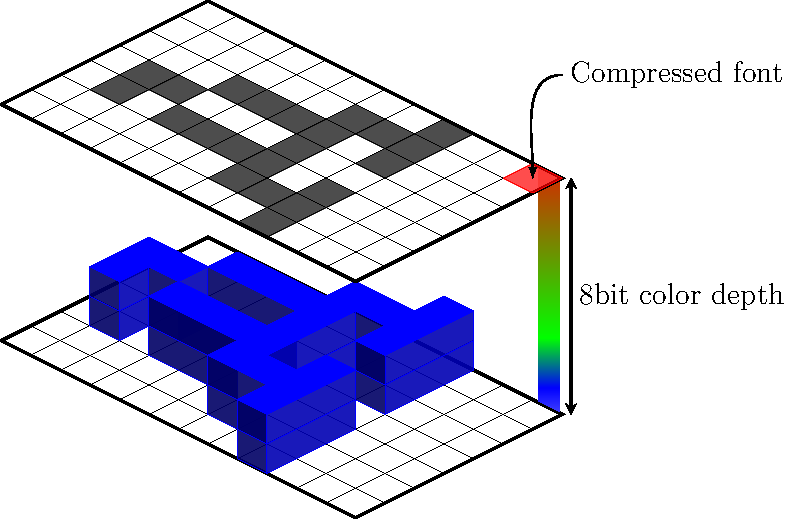
\includegraphics[width=0.6\textwidth]{2-theory/drawing-graphics/graphics/drawingfont8blue.pdf}
	\caption{Double buffer example while writing different images to screen\label{theory:fontgreen}}
\end{figure}
\begin{figure}[H]
	\centering
	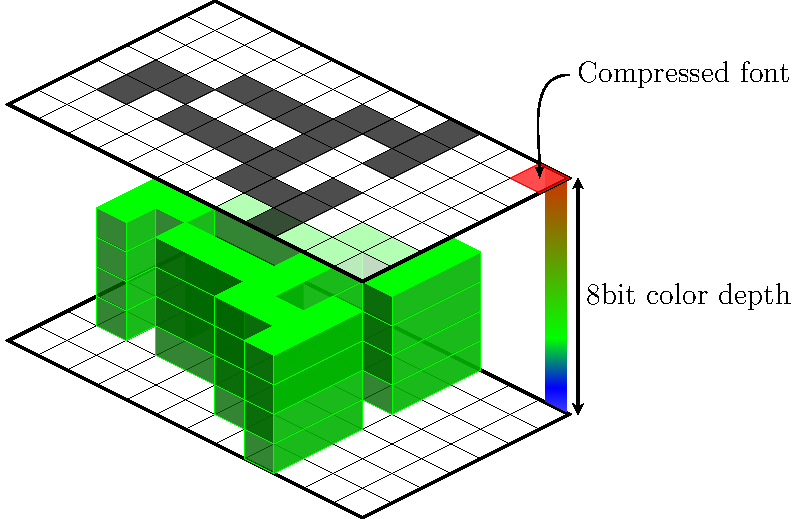
\includegraphics[width=0.6\textwidth]{2-theory/drawing-graphics/graphics/drawingfont8green.pdf}
	\caption{Double buffer example while writing different images to screen\label{theory:fontblue}}
\end{figure}

\begin{figure}[H]
	\centering
	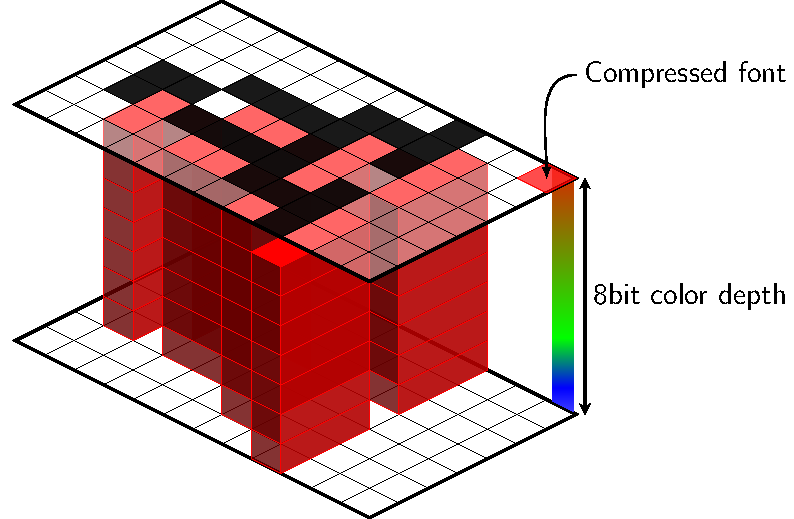
\includegraphics[width=0.6\textwidth]{2-theory/drawing-graphics/graphics/drawingfont8red.pdf}
	\caption{Double buffer example while writing different images to screen\label{theory:fontgreen}}
\end{figure}



